% !TEX root = ../main.tex


\section{Validation}
\label{sec:validation}

One of the attractions of `run to completion' style modelling languages such as \SCXML is their execution semantics which provides a method for animating models to validate their behaviour.
Our approach to \SCXML refinement retains a single \SCXML final model which can be animated using the existing \SCXML animation tools.
However, we would like to validate the developing \UMLB model at intermediate refinement levels.

In previous work~\cite{snook20JSA} we have developed a scenario-based approach to formal modelling using abstract scenarios to validate abstract models.
The method is supported by a `Scenario Checker' tool, based on the \PROB model checker, that allows scenarios to be recorded and then replayed to check that important state has not changed since the original run of the scenario.
The Scenario Checker supports the concept of a controller executing a process in response to changes in the environment which is similar to the run to completion concept addressed in our work here.
Events may be annotated as \emph{internal} to indicate that they should be fired automatically if enabled until none are enabled. 
Internal events may also be prioritised to give a simple representation of process order in the controller (even if it is left non-deterministic in the model).
The user only has to select external events that trigger the controllers responses.
Since our \SCXML derived models already contain an implementation of run to completion the support provided by the Scenario Checker is sufficient to validate this behaviour.
Internal variables that represent the controllers processing (in our case the \SCXML statechart states) can be annotated as \emph{private} so that only controller output is checked during replay.
To help visualise the state of the model, the generated \UMLB state-machine is animated during the scenario validation.
In Figure~\ref{fig:scenarioChecker} we show a previously recorded scenario being played back on the drone model.

\begin{figure}[!h]
	\centering
	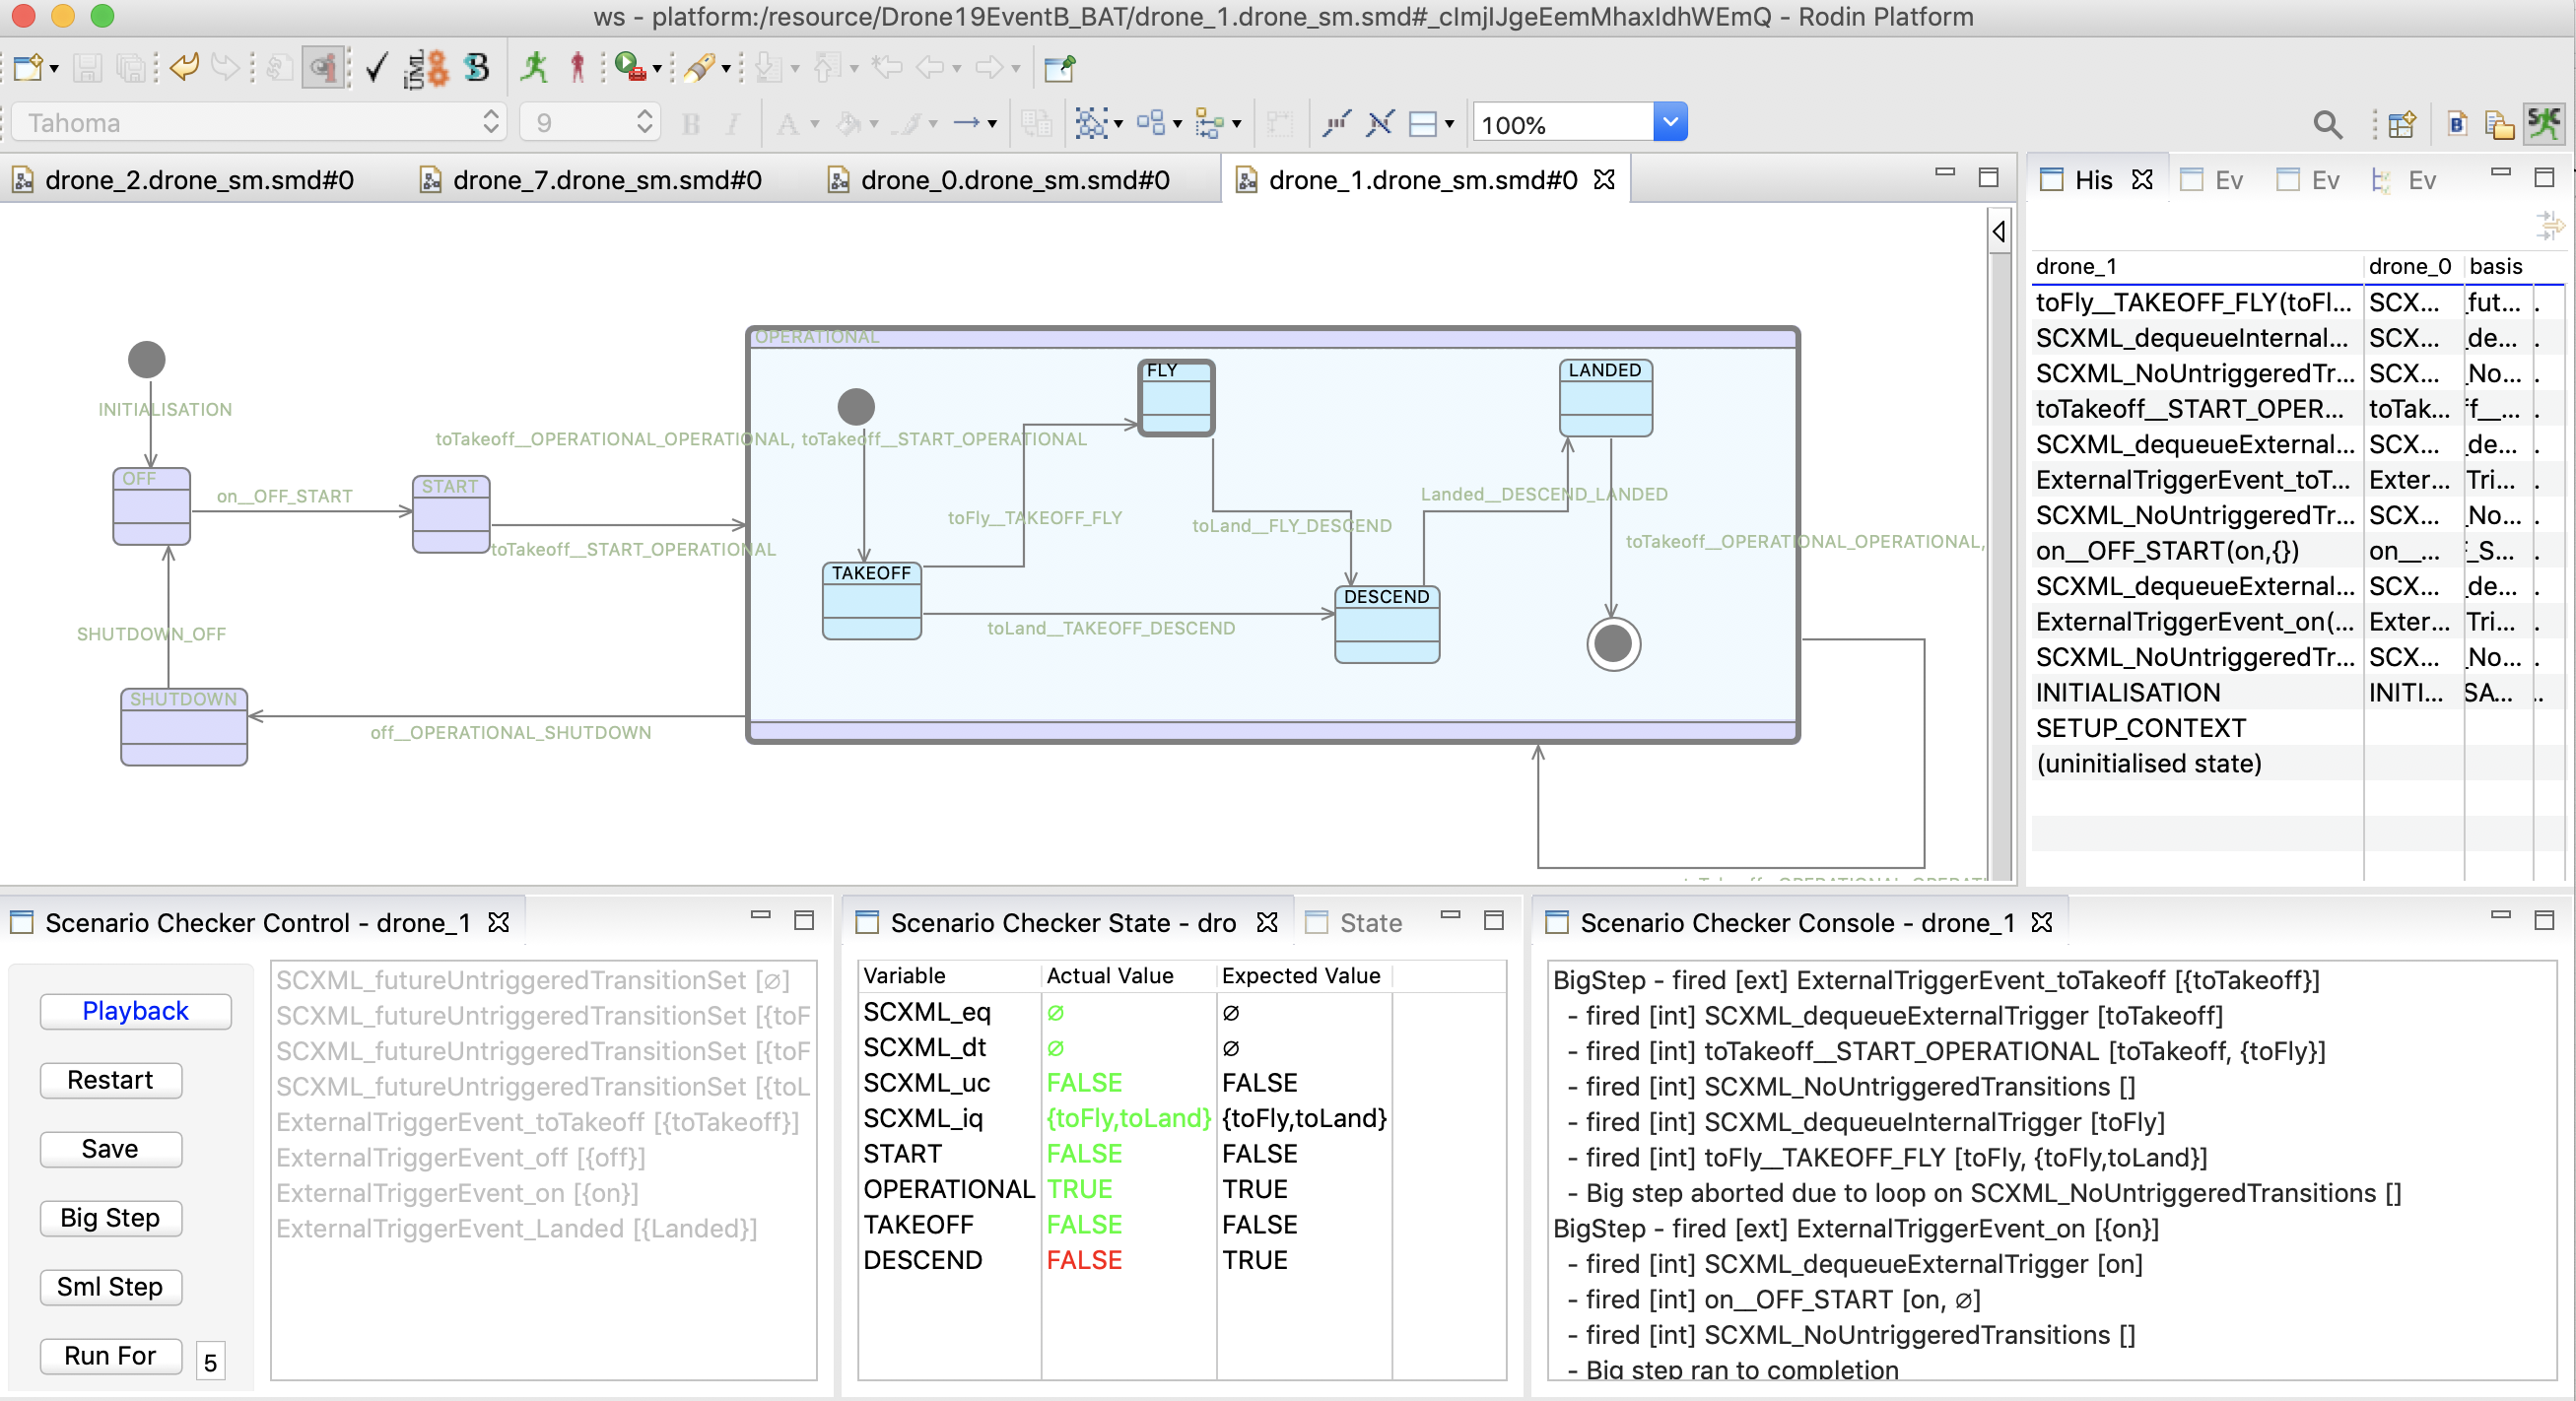
\includegraphics[width=0.90\textwidth, trim=30 50 60 0]{figures/scenarioChecker.png}
	\caption{Using Scenario Checker to validate behaviour}
	\label{fig:scenarioChecker}
\end{figure}

While the scenario checker allows us to animate the expected run to completion behaviour, recall that, unless the transitions have all been finalised (i.e. no further refinement is permitted),  other behaviours are possible due to the non-deterministic completion incorporated in case transition guards are later strengthened. 
The scenario checker allows the run to completion (i.e. internal events) to be overridden in order to explore these behaviours at an abstract level.
 

%%% Local Variables:
%%% mode: latex
%%% TeX-master: "../main"
%%% End:
